\documentclass[10pt]{amsart} 
\usepackage{graphicx} 
\usepackage{float} % necessary for placement of figures
\usepackage{amsmath}
\usepackage{tikz}
\usepackage{pgfgantt} % load Gant chart package
\usepackage{array}
\usepackage[style = authoryear, sorting = nyt, backend = biber]{biblatex}
\addbibresource[location = local, type = file]{C:/Users/bloh356/Google Drive/Library/Library.bib}
% \addbibresource[location = local, type = file]{/Users/bloh356/Google Drive/Library/Library.bib}


\graphicspath {{figures/}}

\title{Uncertainty in reliability parameter estimates: Inclusion in the Generation Expansion Planning (GEP) problem}
\author{Andrew Blohm, Steve Gabriel}
\date{\today}

\begin{document}
\maketitle

\section{Abstract}
What does uncertainty and nonstationarity in gas-fired generator reliability mean for the long-term reliability of our electricity system (and its optimal design)(In progress)? 
We anticipate that traditional methods significantly underestimate the riskiness of investment decisions and thus, overestimate system reliability, which potentially exposes consumers, generators, and system operators to greater risks of unmet demand. 
The contribution of our model to the literature is in the assessment of uncertainty and nonstationarity of the outage rate parameter on the optimal resource mix (as compared to existing methods). 
We anticipate that the composition, costs, and reliability resulting from our method will be quite different than existing methods, which rely on single point parameter estimates. 

\section{Introduction}
Investments in energy production capacity are subject to partial or complete irreversibility (i.e., large, sunk cost that is not particularly fungible) and are large, high-risk investments facing uncertain operating environments (i.e., economic and regulatory uncertainty)\parencite{bakirtzis:2012aa}. 
The Generation Expansion Planning (GEP) problem has been employed extensively to manage these risks while selecting an optimal production portfolio. 
The GEP model determines how best to meet expected future demand through the selection of plant size, production technology, and location, as well as timing over a planning horizon, usually between 10 - 30 years \parencite{hemmati:2013ab}. 
The GEP problem is well studied, from a variety of perspectives including: solution algorithms, incorporation of new production technologies, uncertainty characterization, reliability, time horizon, etc. \parencite{hemmati:2013ab}.

Two approaches are generally used to determine the solution to the GEP: either a centralized or decentralized approach \parencite{bakirtzis:2012aa}.\footnote{The micro-approach incorporates a high amount of model complexity that require operations research or meta-heuristic methods to solve but with the caveate that there is no guarantee that global optimality is achieved. Macro-modeling approaches reduce complexity by ignoring those features and constraints.} 
The centralized approach is appropriate in monopoly situations (i.e., a monopoly utility determining least cost expansion plans) or in deregulated markets by governing or regulating authorities to better design markets and policies \parencite{bakirtzis:2012aa}.
Solution methods for the centralized problem include stochastic dynamic programming (SDP)\parencite{}, non-linear programming (NLP)\parencite{}, evolutionary programming \parencite{}, multi-objective programming \parencite{}, mixed-integer linear programming (MILP) \parencite{}, in addition to other approaches \parencite{}\parencite{bakirtzis:2012aa}.  
[Insert the citations from \cite{bakirtzis:2012aa}.]\footnote{The decentralized approach accounts for the behavior of market participants, usually in a deregulated market framework \parencite{bakirtzis:2012aa}. 
For a more detailed discussion of the decentralized approach the reader is directed to \cite{bakirtzis:2012aa}.} 

Uncertainty incorporation in the generation expansion planning problem has included price volatility, reliability of generation units, load forecast, electricity prices, and costs (i.e., fixed and variable) of each power production technology \cite{hemmati:2013ab, pereira2010decision, pereira2011generation}. 
However, to date, the literature is bereft of an analysis of the effect of uncertainty or trends in the forced outage rate (FOR) parameter on the optimal investment portfolio in the GEP problem. 
Past studies have demonstrated that small changes in the FOR can have significant effects on the reliability of the system \parencite{} (Shirvani (2012))[add citation]. 

There are significant, ongoing changes to the role and deployment of gas-fired generators that are potentially leading to changes in unit reliability. 
Natural-gas fired generators are more frequently ramping, as a result of more renewables, which is having unknown but presumed negative affects on maintenance and reliability [add citation].
At the very least, generators are experiencing increasing O\&M costs as a result of increasing power plant cycling given larger deployments of variable generation, especially for plants designed as baseload units \parencite{nrel:2012aa}.\footnote{Cycling means operating the plant in response to system load requirements (i.e., load following, varying load levels, etc.); as opposed to operating it as a baseload resource \parencite{nerc:2012aa}. Each cycling exposes equipment to pressure and thermal stresses that can damage equipment and subsequently, lead to shorter component life expectancies, higher equivalent forced outage rates (EFOR), and shorter life expectancies \parencite{nerc:2012aa}.} 
These affects are being overlooked by current GEP problem formulations.

Power system adequacy in GEP problems has historically been addressed using deterministic methods, however, over the past few decades probabilistic criteria have largely replaced them.
Deterministic criteria include a planning reserve margin, which could be one of several measures including, setting the reserve margin to the size of the largest generation unit, percentage of system capacity, etc. 
The issue with deterministic approaches (e.g., planning reserve margin) is that they do not account for stochasticity in unit behavior, unit size, etc.
As a result, deterministic methods can lead to either over-investment or inadequate system reliability \parencite{aghaei:2013aa}.

Instead, stochastic methods naturally account for randomness such as unit forced outage rates, size, etc. but at the expense of an increasing computational burden \parencite{aghaei:2013aa}.  
In general, probabilistic metrics measure the duration, intensity or frequency in which demand exceeds the resources available at that time \parencite{dragoon:2006aa}.  	
The adequacy of the deployed resources to meet demand can be incorporated into the GEP problem using: Loss of Load Expected (LOLE)\footnote{The LOLE is the expected number of hours in which demand is not satisfied and is calculated as $LOLE = \sum_{k=1}^S P_k\left(C_T - L_k \right)\times t_k$, where there are S sub-periods and each sub-period is of length $t_k$.}, Loss of Load Probability (LOLP)\footnote{The LOLP is the long-run probability of power system demand exceeding the capacity available \parencite{endrenyi:1978}.  
LOLP can be calculated using daily peak load (i.e. hour demand for a 24 hour period) or using daily peak loads for a 1-year period using a load duration curve \parencite{endrenyi:1978}.}, Loss of Load Cost (LOLC), and Expected energy not served (EENS)\footnote{EENS is the expectation of the energy that the system is not capable of serving and is calculated as the following $EENS = P_k \left(C_T - L_k \right)\times \left(C_T- L_k \right)$.}.\footnote{Given its simplicity LOLE has been extensively used in the past, however, EENS does have certain advantages including that it encompasses the degree of the deficiency, as well as the likelihood \parencite[p622]{murugan2009nsga}.}

In this paper the centralized GEP problem is formulated as a two-stage stochastic mixed integer program.
We incorporate the system reliability measure through the \ldots
The proposed model is evaluated using the IEEE 14 and 30 bus test system \parencite{christie:2009aa}.\footnote{We downloaded the power system data for each of the 14, 30, 57, 188, and 300 bus test systems.}  
[Talk with Jeremy about the appropriate test system].
We consider the forced outage rate of each plant as a random variable, which necessarily impacts system reliability. 
The reliability metric (i.e., LOLE, LOLP, EENS, etc.) are highly sensitive to the EFOR parameter (i.e., a small change in the parameter estimate can lead to large changes in the reliability metric. 
GEP models have not explored the solution space that surrounds the EFOR parameter estimate. 

The rest of this paper is organized as follows: in the second section we discuss the data used in the analysis. 
In the third section, we discuss existing methods for incorporating uncertain parameters, including the forced outage rate, into an optimization framework.
In the fourth section, we propose the mathematical formulation of the two-stage stochastic mixed integer problem. 
In the fifth section, we introduce our case studies before we discuss the results of our model formulation.
In the final section, we discuss some relevant conclusions of our work. 

\section{Data}
A common approach in the literature when developing a new model is to use a well studied data set. 
In the GEP literature this is the IEEE Reliability Test system, which has a number of sizes (i.e., the number of buses in the system) \parencite{billinton:1994aa}. 
We use the IEEE Reliability Test System \ldots [insert system size] \parencite{}. 

\section{Methods}
A number of reviews have been completed that systematically organize the GEP literature.
\parencite{bakirtzis:2012aa, hemmati:2013ab}(Kagiannas et al., 2004; Zhu and Chow, 1997; Hobbs, 1995)\footnote{ Zhu, J., and Chow, M., A Review of Emerging Techniques on Generation Expansion
Planning, IEEE Transactions on Power Systems, Vol.12, No.4, 1997; Hobbs, B.F., Optimization Methods for Electric Utility Resource Planning, European
Journal of Operational Research, 83, 1-20, 1995; 
Kagiannas, A. G., Askounis, D.Th., and Psarras, J., Power Generation Planning: A Survey
from Monopoly to Competition, International Journal of Electrical Power and Energy
Systems, 26, 413-421, 2004}

\cite{bakirtzis:2012aa} incorporates system level reliability using the value of lost load (VLL) in the problem objective function (i.e., mixed-integer linear program) while addressing stochasticity through scenario exploration. 
A simple model is used whereby the equivalent forced outage rate (EFOR) is used to derate the maximum output of each unit \parencite{bakirtzis:2012aa}. 
\cite{tekiner:2010aa} developed a two-stage mixed-integer linear program that addresses stochasticity in the forced outage rates through the development of scenarios using Monte Carlo methods. 

The GEP problem is a large-scale, highly-constrained mixed-integer linear program (MINLP) that requires complete enumeration (i.e., investigation of every combination of assets over the time horizon) to identify the global optimum \parencite{bakirtzis:2012aa}.  
The inability to undertake such an exercise has led to the development of simplifications to reduce the computational load of the problem. 

A common approach to dealing with uncertainties in the GEP framework is Monte Carlo methods \parencite{pereira2010decision}.
Typically, the LOLE and EENS are generated using Monte Carlo techniques \parencite{billinton1996reliability, li2012uncertainty}. 
It is typically built recursively using the Capacity Outage Cumulative Probability Table (COCPT).\footnote{COCPT assumes that the failure of a unit is ``independent of the operating level, system load, and the outage pattern of other units'' (Goel presentation, 2011).} 

Assessing system adequacy using stochastic methods can lead to computational issues given the widely held belief that the GEP is actually a mixed integer non-linear program \parencite{aghaei:2013aa}.
As a result, several methods were developed to assess system adequacy.
\cite{} proposed the 'Z-Method' to evaluate system adequacy in the GEP problem, which replaces the stochastic adequacy assessment metric (i.e., loss-of-load probability (LOLP)) with a new constraint. 
The approach accounts for unit forced outage rates (FOR), system adequacy targets\footnote{In the GEP formulation framework the modeler would select an acceptable level of service (i.e., industry standard is an insufficient capacity with a frequency of 1-in-10 years)\parencite{}. 
The model would then calculate the appropriate reliability statistic using the EFOR (i.e., the number of hours of unit failure as a percentage of all available hours) for each generation unit type and size.}, uncertainty in expected load growth, as well as the size, type and number of units in the production mix \parencite{aghaei:2013aa, \ldots}. 

\section{Model description and mathematical formulation}
Planning and investment in power generation capacity expansion is difficult given the competing objectives for power producers (i.e. minimization of investment costs and maximization of reliability); uncertainty in a number of parameters (i.e.\ costs, demand, regulation), physical and technical constraints, complex mix of regulated and deregulated market structure across the country, and, large and lumpy investments, to name a few. 

We formulate the generation expansion planning problem (GEP) as a two stage, stochastic mixed integer program (SMIP). 
In the first stage the model makes investment decisions while in the second stage the model checks to see that the system meets reliability constraints while in operation.

\section{Nomenclature}
\begin{flushleft}
\textit{Indices and sets}\\
\textit{i} = 1, \ldots, \textit{j} index of the available technologies \\ 
\textit{k} = 1, \ldots, \textit{m} index of the operating modes in the load duration curve [is this the steps?] \\
\textit{n} = 1, \ldots, \textit{N} index of the set of buses \\
\textit{t} = 1, \ldots, \textit{H} index of the periods in the model \\
\end{flushleft}

\begin{flushleft}
\textit{Parameters} \\
$a_i$ = \\
$r$ = discount rate \\
$g_i^t$ = existing capacity of technology \textit{i} at time \textit{t} \\
$ic_{nt}$ = investment cost of technology \textit{i} at time \textit{t} \\
$j_{nt}$ is the average capacity (MW) of \textit{nt} \\
$L_i$ = lifetime of technology alternative \textit{i} \\
$oc_{ik}^{t}$ = marginal cost of production for technology \textit{i} during load block \textit{k} at time \textit{t} \\
$\rho_{i}^{t}$ = duration of load block \textit{k} at time \textit{t} \\
\end{flushleft}

\begin{flushleft}
\textit{Variables}[will separate into continuous and binary later] \\
$q_{ik}^{t}$ = active power generation of new generating units by technology \textit{i} for load block \textit{k} at time \textit{t} \\
$q_{ik}^{t}$ = active power generation of new generating units by technology \textit{i} for load block \textit{k} at time \textit{t} \\
$w_{i}^{t}$ = total capacity of technology \textit{i} at time \textit{t} \\
$x_{nt, n}$ = integer variable that represents the number of nt at node \textit{n} \\
\end{flushleft}

\begin{equation}
min_{x,y,w} \sum_{t=1}^{H}\bigg[\bigg(\sum_{i=1}^{j} ic_{nt, n}^{t}\cdot \big(x_{i}^{t} - x_{i}^{t-1}\big) + \sum_{i=1}^{j} \sum_{k=1}^{m} oc_{i}^{kt}\cdot \rho_{kt}^{t}\cdot q_{ik}^{t} \bigg)\bigg((1+ r)^{t-1}\bigg)^{-1}\bigg]
\end{equation}

The deterministic version of the model: 
\begin{equation}\label{Lopez.2007}
min_{x,y,w} \sum_{n} \sum_{nt} ic_{nt}\cdot j_{nt}\cdot x_{nt, n}  + \sum_{k} \bigg(\sum_{h}\sum_{et}oc_{et}\cdot q_{k,et,h} + \sum_{n}\sum_{nt} oc_{nt}\cdot q_{k,nt,n}\bigg) 
\end{equation}

The budget constraint
\begin{equation}
\sum_{n}\sum_{nt} ic_{nt}\cdot j_{nt}\cdot x_{nt, n} \leq B
\end{equation}

Nodal balance constraints:

Power flow constraints:

In Equation \ref{Lopez.2007} I need to weight the operating costs by the capacity factor for each technology.

\subsection{Load model description}
The system load for each period is represented using a step-wise load duration curve. 
Demand varies across the year using a load duration curve representation that decomposes annual demand into several load segments. 
The number of steps was chosen to accurately represent the load duration curve across the hours.
\subsection{Energy balance constraints}
\subsection{Unit operating cost constraints}
\subsection{Annual budget constraints}
\subsection{Binary constraints}
\subsubsection{Maximum construction limit \nopunct}
This constraint is a maximum allowable number, capacity, or investment amount for new generation sources to be built during period \textit{t} given limited resources (i.e., capital, manpower, space, etc.). 
\subsubsection{LOLP constraint \nopunct}
To ensure that adequacy requirements (i.e., minimum level of service) are maintained the GEP problem formulation typically includes reliability constraints.\footnote{Reliability and adequacy are considered early in the planning process, typically well before stability and fault analysis. These factors are a necessary component of any long-term planning process; otherwise, there is no guarantee of having adequate supply to meet system demand.}\footnote{The determination of the adequate generation supply capacity can be divided into two areas: static and operating capacity requirements \parencite{billinton1984reliability}.
In this study, we focus on the static capacity requirement, which is the capacity that must be planned and installed in advance of system demand (i.e., as a part of a long-term planning process) \parencite{billinton1984reliability}.
Static capacity must be able to provide for outages and regularly scheduled maintenance, in addition to anticipated load growth \parencite{billinton1984reliability}.
Operating capacity, which we mention only for completeness, determines the capacity necessary to meet actual short-term load and is used in different frameworks, such as unit commitment problems \parencite{billinton1984reliability}.}
\begin{equation}
\textit{lolpc}_{t} \leq \textit{lolps}_{t} \forall t \in T 
\end{equation}

The $\textit{lolpc}_{t}$ is the loss-of-load probability at stage \textit{t} and $\textit{lolps}_{t}$ is the loss-of-load probability limit (i.e., the reliability target selected by the user) \parencite{dragoon:2006aa}. 
The equivalent Z constraint is \ldots
\subsection{Computational, convergence, and feasibility issues}
[Insert description of the computer used to solve]
[Insert description of the number of variables and equations]
\cite{bakirtzis} used a convergence tolerance of 0.25\% with their model taking between 7 and 18 minutes to solve. 

\section{SMIP GEP: Case study}
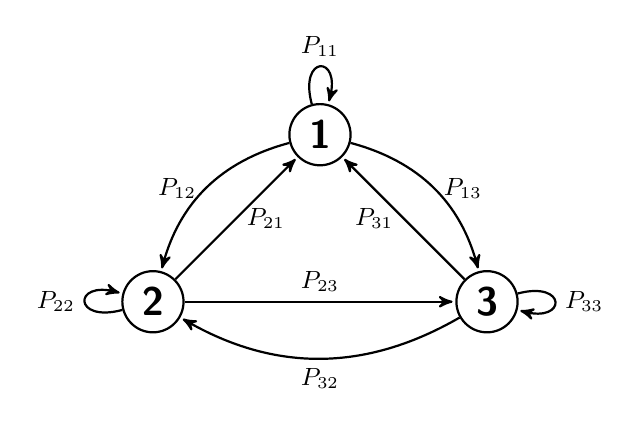
\begin{tikzpicture}[->,>=stealth',shorten >=1pt,auto,node distance=3cm,
                    thick,main node/.style={circle,draw,font=\sffamily\Large\bfseries}]
	\node[main node](1){1};
	\node[main node](2)[below left of=1]{2};
	\node[main node](3)[below right of=1]{3};

	\path[every node/.style={font=\sffamily\small}]
	 (1) edge [bend left] node[right] {$P_{13}$} (3)
	 edge [bend right] node[left] {$P_{12}$} (2)
	 edge [loop above] node[above] {$P_{11}$ }(1)
	 (2) edge node [right] {$P_{21}$} (1)
	 edge node [above] {$P_{23}$} (3)
 	 edge [loop left] node[left] {$P_{22}$} (2)
	 (3) edge node [left] {$P_{31}$} (1)
	 edge [loop right] node[right]{$P_{33}$} (3)	
	 edge [bend left] node[below]{$P_{32}$}(2);
\end{tikzpicture}

\section{Results}
The proposed model is evaluated using the \ldots bus IEEE Reliability test network \parencite{}.
The system has \ldots nodes with total installed demand and capacities as defined in Table \ref{}. 
We display other assumptions, such as the fuel cost and variable operations and maintenance costs in Table \ref{}.
The average load of the system is \ldots with a peak load of \ldots.

The load duration curve \ldots
We have \ldots scenarios for the load growth: \ldots 

[Insert model parameterization discussion here]

\section{Discussion}




	 






\printbibliography
\end{document}

